% This must be in the first 5 lines to tell arXiv to use pdfLaTeX, which is strongly recommended.
\pdfoutput=1
% In particular, the hyperref package requires pdfLaTeX in order to break URLs across lines.

\documentclass[11pt]{article}

% Remove the "review" option to generate the final version.
\usepackage[]{acl}

% Standard package includes
\usepackage{times}
\usepackage{latexsym}

% For proper rendering and hyphenation of words containing Latin characters (including in bib files)
\usepackage[T1]{fontenc}
% For Vietnamese characters
% \usepackage[T5]{fontenc}
% See https://www.latex-project.org/help/documentation/encguide.pdf for other character sets

% This assumes your files are encoded as UTF8
\usepackage[utf8]{inputenc}

% This is not strictly necessary, and may be commented out,
% but it will improve the layout of the manuscript,
% and will typically save some space.
\usepackage{microtype}

\usepackage{graphicx}
\graphicspath{ {./images/} }

\usepackage{longtable}
\usepackage{booktabs}

% If the title and author information does not fit in the area allocated, uncomment the following
%
%\setlength\titlebox{<dim>}
%
% and set <dim> to something 5cm or larger.

\title{Fine-tuning vs prompting in adaptation of language model for multi-label classification}

% Author information can be set in various styles:
% For several authors from the same institution:
% \author{Author 1 \and ... \and Author n \\
%         Address line \\ ... \\ Address line}
% if the names do not fit well on one line use
%         Author 1 \\ {\bf Author 2} \\ ... \\ {\bf Author n} \\
% For authors from different institutions:
% \author{Author 1 \\ Address line \\  ... \\ Address line
%         \And  ... \And
%         Author n \\ Address line \\ ... \\ Address line}
% To start a seperate ``row'' of authors use \AND, as in
% \author{Author 1 \\ Address line \\  ... \\ Address line
%         \AND
%         Author 2 \\ Address line \\ ... \\ Address line \And
%         Author 3 \\ Address line \\ ... \\ Address line}

\author{Sergey Grebenkin \\
  AI Professional Program \\
  Stanford Online Course \\
  \texttt{sergey.grebenkin@gmail.com} \\\And
  Georgii Shushuev \\
  AI Professional Program \\
  Stanford Online Course \\
  \texttt{shyshyev@gmail.com}
}

\begin{document}
\maketitle
\begin{abstract}
In this study, we examined the effectiveness of two approaches to multi-label text classification. The first approach is fine-tuning a simple encoder model, and the other is prompting an LLM. The final encoder layer of pre-trained models BERT, RoBERTa, and ELECTRA, along with the classification head, were retrained on a well-curated dataset. The prompt engineering approach for Chat GPT models was used to compare performance with the aforementioned models. It was shown that fine-tuning encoder models achieves higher quality than complex prompting without fine-tuning when using an inexpensive proprietary model like GPT-4o-mini. However, when using a powerful model like GPT-4o, the prompt shows high performance, surpassing fine-tuned models, however, this is not the subject of the given article.

It was also hypothesized that it is always possible to develop a prompt that will outperform any fine-tuned model for a specific task. This was confirmed on GPT-4o (but not on GPT-4o-mini). This explores the potential of prompt engineering, arguing that with sufficient effort and understanding of the task, prompts can be created that allow large models to achieve superior performance compared to fine-tuned models, especially for well-defined tasks. Some studies, such as \cite{huggingface}, show that this can be an effective approach to narrowing down the solution to a simpler mode. Nevertheless, the usage of GPT-4o is far more expensive than GPT-4o-mini. Also, GPT-4o-mini from its side is more expensive than BERT, RoBERTa, ELECTRA. This is why it's also important to understand when using BERT-like models makes more sense both from budget and quality standpoint.

\end{abstract}

\section{Introduction}

The growing use of natural language understanding (NLU) for process automation has led to increased interest in methods that allow machines to interpret and execute complex instructions given in free text. One specific use case in the medical field is the automatic interpretation of doctors' prescriptions, which requires converting unstructured text into a structured format that machines can act upon. While fine-tuning pre-trained language models has been the traditional approach to adapting models for specific tasks like classification or named entity recognition (NER), prompting has emerged as a flexible alternative, particularly with the advent of large language models (LLMs) like GPT-4.

\section{Prior Literature}

The growing use of natural language understanding (NLU) for process automation has led to increased interest in methods that allow machines to interpret and execute complex instructions given in free text. One specific use case in the medical field is the automatic interpretation of doctors' prescriptions, which requires converting unstructured text into a structured format that machines can act upon. While fine-tuning pre-trained language models has been the traditional approach to adapting models for specific tasks like classification or named entity recognition (NER), prompting has emerged as a flexible alternative, particularly with the advent of large language models (LLMs) like GPT-4.

This literature review compares the efficacy of fine-tuning and prompting for structured output tasks that do not involve free-form text generation, such as converting textual prescriptions into predefined grammar or structured data formats like JSON. We explore whether fine-tuning consistently outperforms prompting or if a well-engineered prompt can yield competitive or even superior results without the need for extensive labeled datasets or model retraining. Our analysis focuses on key NLP tasks like sentiment analysis, multi-label classification, and information extraction, questioning whether prompting alone can rival fine-tuning in non-generative contexts.

The review also addresses the trade-offs between these methods and their implications for future NLP applications. The findings aim to guide researchers and practitioners in selecting the most appropriate approach for tasks where structured, non-generative outputs are required.

\subsection{General problem / Task definition}
  
Natural language understating very often is an essential task for process automation. When we are talking about "automation" we are talking about something that can be performed without humans. At our job, we faced a task when it was necessary to understand what the doctor asked to perform in the prescription. There could be many different wishes about the ways how the doctor wants the treatment to be performed. To automatically create such treatment, or to automatically check if the treatment was created properly we need to make the machine understand what the doctor asks. So we need to create some structured language to explain the machine doctor's wishes. 

Although there are many different preferences for how the doctor wants the treatment to be carried out, their number is finite, and the parameters of each preference are also finite. So if we can create some grammar that can describe any doctor's wishes, it means that we can make the machine understand what the doctor asks. The task here is only to create an algorithm that can convert free text doctor's prescriptions to this grammar. 

In the case of humans, it takes several years of education to be able to do it. In the case of machines, it should be comprehensive instruction that explains all the ways how doctors can ask for some actions. Or it should be labeled a dataset of examples of how free text prescriptions convert to the grammar? Or both? What model is more effective to create such a conversion algorithm? It is the questions that we faced and this literature review has a goal to find the answer. It is important to remark that it is a quite broad problem that is actual almost in any field where free text instructions exists. Even if we imagine the AI hairdresser the client, if he hasn't a photo what result does he want to get, will explain in a free text way how he wants his hair cut.

In the domain of natural language processing (NLP), there are multiple strategies for leveraging large language models (LLMs) to solve a variety of tasks. Two key approaches are fine-tuning and prompting. While fine-tuning has traditionally been the go-to method for adapting pre-trained models to specific tasks, prompting has gained considerable attention due to its simplicity and flexibility, especially when working with very large language models like GPT-4.

This literature review focuses on tasks that do not require free-form text generation but instead involve more structured outputs, such as classification, named entity recognition (NER), information extraction, and text-to-structured-data transformations (e.g., converting unstructured text into a JSON format - the very grammar that was mentioned earlier). These tasks often require models to identify patterns, label data, or map textual inputs to predefined structures, which can be approached in several ways.

Historically, tasks like sentiment analysis or multi-label/multi-class classification have been effectively solved by fine-tuning models such as BERT on task-specific datasets. Fine-tuning allows models to adapt deeply to the task at hand by adjusting all their parameters based on the labeled data available. However, this approach can be challenging when datasets are scarce or tasks are highly domain-specific.

In such cases, prompting presents an alternative. With a well-designed prompt, even a general-purpose LLM (e.g., GPT-4) can be leveraged to produce high-quality annotations for tasks where large labeled datasets do not exist. For example, one might craft a detailed prompt that instructs the model on how to label text or convert it into structured data (the grammar). This prompt-based approach can serve as a data augmentation technique, where the LLM is used to generate a synthetic dataset, which can then be used to fine-tune a smaller, task-specific model.

The key question this review seeks to explore is whether fine-tuning can consistently outperform prompting in tasks where no free-text generation is required. If a well-engineered prompt can achieve high accuracy without the need for extensive dataset creation and model retraining, then prompt-based methods could offer a more efficient path to solving classification and extraction problems. However, it remains unclear whether improving prompts alone can lead to better performance than fine-tuning, especially as prompt engineering requires considerable trial and error, and the potential of fine-tuning remains powerful when sufficient task-specific data is available.

Thus, this review will examine the comparative advantages of each approach in non-generative tasks, particularly focusing on questions like:

\begin{itemize}
    \item Can fine-tuning always outperform prompting when data is available, or can prompt-based LLM methods be equally effective?
    \item Are there specific tasks or conditions where prompting could replace the need for fine-tuning entirely?
    \item What trade-offs exist between these methods, and how might this influence the choice of approach in future NLP applications?
\end{itemize}

\subsection{Summary of Articles}

\subsection{Language Models are Few-Shot Learners}
We would like to start with an article that, by its appearance, indicated that large language models can compete with fine-tuned state-of-the-art solutions. At the time of writing the paper, one of the authors (Jared Kaplan) worked at OpenAI and is now Chief Science Officer at Anthropic ~\cite{LMFSL:2020}.

\subsubsection{Key Points}
Research Objective: The study demonstrates that scaling up language models significantly improves their performance in few-shot learning tasks, sometimes even becoming competitive with fine-tuning approaches.

GPT-3 Model: The authors trained GPT-3, an autoregressive language model with 175 billion parameters, which is 10 times larger than previous models. GPT-3 shows strong results on many NLP datasets, including translation, question-answering, and close tasks.

Training Methods:
\begin{itemize}
    \item Zero-Shot: The model performs tasks without any examples, using only a textual description of the task.
    \item One-Shot: The model is given one example of the task before performing it.
    \item Few-Shot: The model is given several examples of the task before performing it.
    \item Fine-Tuning: updates the weights of a pre-trained model by training on thousands of
supervised labels specific to the desired task.
\end{itemize}
Results:
\begin{itemize}
    \item GPT-3 shows significant performance improvements with increased model size.
    \item In few-shot tasks, GPT-3 sometimes outperforms models fine-tuned on specific tasks.
    \item On some tasks, GPT-3 still lags behind fine-tuned models, especially in zero-shot and one-shot settings
\end{itemize}
\subsubsection{Mentions of BERT}
Most interesting for our goal is a comparison with the fine-tuned BERT model:
\begin{itemize}
    \item The paper compares GPT-3’s performance with BERT-Large on the SuperGLUE dataset. BERT-Large was fine-tuned on the SuperGLUE training set (125K examples), as well as on MultiNLI (392K examples) and SWAG (113K examples), totaling 630K fine-tuning examples.
    \item GPT-3’s performance in the few-shot setting is compared to BERT-Large and BERT++, showing that GPT-3 with one example in context (one-shot) and eight examples (few-shot) achieves results comparable to fine-tuned BERT models.
\end{itemize}
Results on SuperGLUE:
\begin{itemize}
    \item On SuperGLUE tasks, GPT-3 in the few-shot setting shows results close to state-of-the-art, held by fine-tuned models like BERT-Large.
    \item In tasks such as COPA and ReCoRD, GPT-3 achieves near-SOTA performance in one-shot and few-shot settings, falling only slightly short of the fine-tuned T5 model with 11 billion parameters.
\end{itemize}
Limitations and Weaknesses:
\begin{itemize}
    \item The paper notes that GPT-3 sometimes falls short of fine-tuned models like BERT on tasks requiring the comparison of two sentences or text snippets (e.g., WiC and RTE).
    \item GPT-3 also shows weaker results on tasks that benefit from bidirectional architectures, which is a strength of BERT.
\end{itemize}
\subsubsection{Conclusion}
At the time of writing, approaches based on BERT had already been developed long ago and were very strong, and the GPT-3, as we now know, was far from being the smartest model, and even it had already achieved the quality of the state-of-the-art models in some tasks after just a few shots.

\subsection{Prompt Programming for Large Language Models: Beyond the Few-Shot Paradigm}
The next article is about the prompting strategy, namely that a zero-shot is better than a few-shot. This article is interesting for us because we reached the same conclusion independently in our task while working with the prompt ~\cite{PPfLLM:2021}.
\subsubsection{Key Points}
Research Objective: The study explores methods for effectively controlling and evaluating large language models like GPT-3 through prompt programming, emphasizing the potential of zero-shot prompts over few-shot prompts.

Prompt Programming: The authors argue that few-shot examples often serve to locate an already learned task rather than teaching the model the task during runtime. They propose that prompt programming, especially using zero-shot prompts, can be more effective.

In this article added the one new training method: 
\begin{itemize}
    \item Metaprompt Programming: Introducing the idea of a metaprompt that seeds the model to generate its own natural language prompts for a range of tasks.
\end{itemize}
Results:
\begin{itemize}
    \item Zero-Shot Prompts: The study finds that zero-shot prompts can match or even exceed the performance of few-shot prompts with minor prompt engineering.
    \item Task Location: Few-shot examples primarily help the model locate the task within its existing knowledge rather than learning it anew.
    \item Prompt Engineering: Simple changes in prompt formatting can significantly improve performance, indicating that GPT-3’s zero-shot capabilities were underestimated.
\end{itemize}
\subsubsection{Conclusion}
The study emphasizes the importance of prompt programming in leveraging the full potential of large language models. It suggests that zero-shot prompts and metaprompt programming can significantly enhance the performance and flexibility of models like GPT-3, potentially surpassing the need for few-shot learning in many cases. The authors call for further research into automated prompt generation and more sophisticated benchmarking methods to better evaluate and utilize these models.

\subsection{Fine-tuning and prompt engineering for large language models-based code review automation}
This paper ~\cite{FTaPE:2024} is interesting for us because consists detailed review and comparison of using LLM techniques in a quite close task for us. 
\subsubsection{Key Points}
Research Objective: The study investigates the performance of code review automation using large language models (LLMs) based on two approaches: fine-tuning and prompt engineering.

Methods:
\begin{itemize}
    \item Fine-Tuning: Further training the model on a specific code review dataset.
    \item Prompt Engineering: Providing explicit instructions to guide the model’s generation process without requiring a specific code review dataset.
\end{itemize}
\subsubsection{Results}
Fine-Tuning:
\begin{itemize}
    \item Fine-tuning GPT-3.5 with zero-shot learning achieves 73.17\%–74.23\% higher Exact Match (EM) compared to the approach by Guo et al.
    \item Fine-tuning GPT-3.5 with zero-shot learning achieves 63.91\%–1100\% higher EM compared to non-fine-tuned GPT-3.5.
\end{itemize}
Prompt Engineering:
\begin{itemize}
    \item GPT-3.5 with few-shot learning achieves 46.38\%–659.09\% higher EM compared to zero-shot learning.
    \item Using a persona in prompts reduces EM by 1.02\%–54.17\%.
\end{itemize}
\subsubsection{Conclusions}
\begin{itemize}
    \item Fine-Tuning: Recommended for achieving the highest performance in code review automation.
    \item Few-Shot Learning: When data is insufficient for fine-tuning (e.g., cold-start problem), few-shot learning without a persona should be used.
\end{itemize}


\subsection{Large Language Models for Text Classification: From Zero-Shot Learning to Instruction-Tuning}
One of the most obvious tasks for comparison prompted LLM with fine-tuned BERT-like models is text classification. But LLMs can also be compared with each other based on how they cope with this task and which approaches to their use are best suited for this ~\cite{LLMfTC:2024}. The article is fresh, includes a comparison with GPT-4o and even here BERT-like approaches for classification show themselves to be on the level.
\subsubsection{Introduction}
The article explores the application of large language models (LLMs) to supervised text classification, focusing on stance detection. It compares ten models ranging from 86 million to 1.7 trillion parameters across four training regimes: zero-shot learning, few-shot learning, fine-tuning, and instruction-tuning.
\subsubsection{Key Findings}
Zero-shot Learning:
\begin{itemize}
    \item Advanced LLMs can perform text classification without any task-specific training by leveraging their pre-trained knowledge.
    \item GPT-4o achieved high accuracy in zero-shot settings, outperforming many fine-tuned models.
\end{itemize}
Few-shot Learning:
\begin{itemize}
    \item Adding a few labeled examples alongside prompts can sometimes improve performance but is highly sensitive to the choice of exemplars.
    \item Performance varies significantly depending on the exemplars provided.
\end{itemize}
Fine-tuning:
\begin{itemize}
    \item Fine-tuning smaller models can be competitive due to their relatively high accuracy and low cost.
    \item Larger models like GPT-3 Davinci showed significant improvements with fine-tuning, especially with more training data.
\end{itemize}
Instruction-tuning:
\begin{itemize}
    \item Instruction-tuned models can handle complex tasks by combining the strengths of prompting and fine-tuning.
    \item Llama3-70B showed comparable performance to GPT-4o after instruction-tuning.
\end{itemize}
Results:
\begin{itemize}
    \item Zero-shot and Few-shot Learning: Larger models like GPT-4o and Llama3-70B performed exceptionally well in zero-shot settings.
    \item Fine-tuning: Smaller models like BERT and DeBERTa showed competitive performance when fine-tuned on larger datasets.
    \item Instruction-tuning: Llama3-70B achieved high accuracy in complex tasks involving structured data like comment-reply threads.
\end{itemize}
Recommendations
\begin{itemize}
    \item Model Selection: Depends on the task complexity, document length, number of documents, and available resources.
    \item Zero-shot/Few-shot Learning: Suitable for small datasets or when labeled data is scarce.
    \item Fine-tuning: Effective for larger datasets with sufficient annotated examples.
    \item Instruction-tuning: Ideal for complex tasks requiring detailed instructions and handling structured data.
\end{itemize}

\subsubsection{Conclusion}
LLMs offer powerful tools for text classification, with zero-shot and instruction-tuning opening new possibilities for social scientific research. The choice of model and training regime should be guided by the specific requirements of the task and available resources.


\subsection{Fine-tuning after Prompting: an Explainable Way for Classification}

In the paper Zhezhong Wang at al. investigates a hybrid approach to use the pre-trained language models (PLMs) for classification tasks, combining the strengths of both fine-tuning and prompting. The authors introduce a method called F\&P, that "attains performance on par with Fine-tuning while
preserving the outstanding explainability inherent to Prompting methods". In this method, a prompt is used to guide the PLM's predictions, and a linear classifier is fine-tuned on the model’s output to improve classification accuracy. The classifier's weights are then used to create a "verbalizer," mapping the model's output words to their corresponding classes. Authors also introduce an optimisation of F\&P method called Fine-tuning and AUTOPROMPT (F\&AP) leveraging AUTOPROMPT (Shin et al., 2020).

The key advantage of F\&P is that both the prompt and verbalizer are based on natural language, making the process more explainable to humans compared to traditional fine-tuning methods. Experiments on English and Chinese datasets, using benchmarks such as GLUE and CLUE, demonstrate that the F\&P and F\&AP methods achieve superior performance with fine-tuning in terms of avg F1 score while maintaining greater interpretability. Additional parameters are not added to the model, therefore the size is not changed. Furthermore, the authors argue that this approach offers a balance between explainability and accuracy, suggesting its potential in practical applications where model transparency is essential.

\subsection{No More Fine-Tuning? An Experimental Evaluation of Prompt
Tuning in Code Intelligence}

In this article Wang at al. investigate the use of prompt tuning as an alternative to traditional fine-tuning methods for code intelligence tasks. The study measures the performance of prompt tuning and fine-tuning on three tasks: defect detection, code summarization, and code translation, using pre-trained models such as CodeBERT and CodeT5. Prompt tuning modifies model inputs by adding task-specific prompts, allowing it to align more closely with the model’s pre-training objectives.

The experiments show that prompt tuning consistently outperforms fine-tuning across all tasks, particularly in low-resource scenarios where data is scarce. It also significantly improves BLEU scores in code summarization by over 26\%. Different prompt templates and verbalizer choices can affect the performance, and prompt tuning shows more advantages with smaller pre-trained models.

The authors suggest that prompt tuning is a promising method for code intelligence, especially in cases with limited training data, and recommend further research into optimizing prompt design for various tasks.

\subsection{Comparison of Prompt Engineering and Fine-Tuning Strategies in Large Language Models in the Classification of Clinical Notes}

In the article Zhang at al. evaluate different methods to classify clinical notes, particularly focusing on identifying metastatic cancer. They compare the effectiveness of prompt engineering and fine-tuning strategies across several language models, including GPT-3.5, GPT-4, and Llama-7B, against BERT-based models and human annotators.

The study shows that GPT-4 outperformed GPT-3.5 and Llama-7B in classification tasks, demonstrating superior accuracy and robustness across different prompts and token sizes. Prompt engineering, especially structured prompts, showed strong performance in zero-shot learning scenarios, often outperforming fine-tuning models.

Fine-tuning Llama-7B yielded moderate results, but did not surpass GPT-4’s performance, particularly in tasks requiring precision. One-shot learning provided little to no advantage over zero-shot learning in most cases.

GPT-4's performance remained stable even when keywords were removed or token counts reduced, showing resilience in handling incomplete or sparse data.

The article concludes that using effective prompt engineering, large language models like GPT-4 can potentially replace domain-specific models like PubMedBERT in biomedical tasks, offering comparable or superior performance without extensive fine-tuning.

\section{Compare and Contrast}

In the above-mentioned articles the fine-tuning and prompting are considered two important methods for models adaptation for the given task. Mainly pre-trained models were used in the studies. The results are dependent on the task and the models used. However, there are some general conclusions that could be done based on them.

While majority of the articles highlight a prompting as the superior methods for enhancing the model performance, some of the studies show that fine-tuning could be a better option in some specific applications. Pornprasit et al. proves fine tuning achieves better exact match score compared to non fine-tuned models. Few-shot prompting shows improvement in specific context.

It should be noted that there is some contradiction in the articles by Reynolds et al. (2021) and Pornprasit et al. (2024), one says that the few-shot prompting is better than the zero-shot prompting, while in the other the key idea is that if done correctly the zero-shot is no worse or even better than the few-shot. Probably this could be attributed to the different years of studies and some conclusions from Reynolds et al. (2021) could not be applied to modern models.

One of the approaches that is worth mentioning is the combined usage of both fine-tuning and prompting called F\&AP, evaluated by Wang et al. While not being a game changer, for some applications it could be the best option as it leads to avg F1-score improvement on GLUE from 1\% for RoBERTa-based models up to 3.6\% for OpenAI GPT.

As it turns out, fine-tuning could be a good option when using pre-trained model for a specific task. Also, On the other side, fine-tuning could be computationally expensive in some situations and requires labeled datasets. Every time it's recommended to fit the model for a new type of task separately.

To sum up, the pros of fine-tuning are deep adaptation to specific task, high-performance on well-defined datasets for specific domain. The cons are necessity of labeled datasets and computational complexity. The pros of prompting are quick implementation, large datasets are not required. On the other site the cons could be high dependence of prompt quality.

\section{Data}

In this study, we will utilize the dataset to evaluate the performance of fine-tuning and prompting methods for structured output tasks. The selected dataset covers a text classification tasks, including multi-label classification, to provide a comprehensive assessment of the models’ capabilities.

The dataset for the task should support multiple labels for each text instance. A good source for such datasets is Kaggle, where various multilabel classification datasets are available. One example is the ArXiv Paper Abstracts dataset \cite{kaggle}. This dataset includes abstracts of academic papers with multiple labels corresponding to different research topics, providing a challenging testbed for our models. Another one is \cite{kaggle2} to classify the research papers based on Abstract and Title.

In real-world production environments, labeled datasets are often scarce and expensive to create. This poses a significant challenge for training and fine-tuning models. To address this issue, we propose leveraging large language models (LLMs) with well-crafted prompts to generate labeled data. By using prompt-based methods, we annotate unlabeled data efficiently, reducing the need for extensive manual labeling efforts. This approach not only saves time and resources but also enables the rapid adaptation of models to new tasks and domains.

Although our focus is on structured output tasks, we use classification datasets to illustrate our approach. For example, sentiment analysis is a classification task that can be effectively solved by fine-tuning BERT. When dealing with non-standard classification tasks where labeled datasets are unavailable, a well-designed prompt for a powerful LLM (e.g., GPT-4) can be used to annotate large amounts of text, which can then be used to fine-tune a model.

The key idea is that tasks not requiring free-form text generation—such as multi-label/multi-class classification, named entity recognition (NER), information extraction, and even converting free text to a structured JSON format—can be addressed by fine-tuning models that do not generate text. While it might seem convenient to solve the task of converting text to a structured JSON format by describing the transformation rules in a prompt, essentially, we are asking the LLM to perform multiple classification/NER tasks.

Structured output tasks often involve transforming unstructured text into a predefined format, such as JSON. This transformation can be broken down into several smaller tasks, such as identifying entities, classifying text segments, and assigning labels. Multi-label classification is a specific type of structured output task where each text instance can belong to multiple categories simultaneously. By using multi-label classification datasets, we can simulate the complexity of real-world structured output tasks and evaluate how well our models can handle multiple labels and categories.

In this paper we use the labeled dataset of orthodontic instructions by doctor. The size of the dataset is 5451 entries. It contains the mapping of orthodontic instruction to json with the list of 20 mentioned orthodontic-specific parameters like alignment, bite, crowding, midline e.t.c. The structure looks like follows - if alignment is mentioned directly or in other words, then the resulting json contains the pair { "alignment": 1 }, otherwise, if alignment is not mentioned, then the pair would be { "alignment: 0 }.

To prepare dataset for classification task we converted each json representation to vector of 20 parameters, where each index value corresponds to each parameter, sorted alphabetically. Since the teeth alignment corresponds to the first parameter, if it mentioned in doctor instructions and other parameters not, the vector would look like [1, 0, ..., 0].

The distribution of doctor instructions sizes looks as follows.
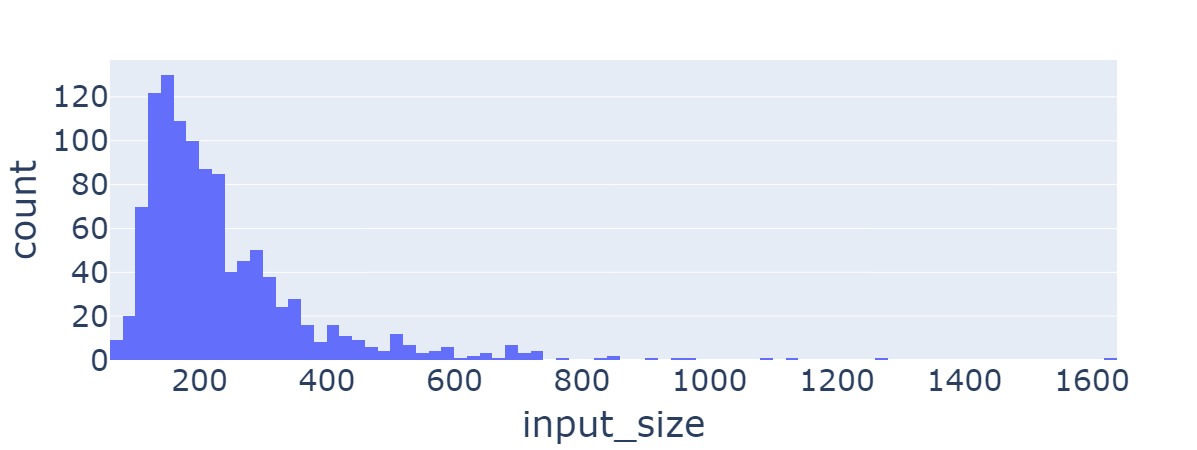
\includegraphics[scale=0.2]{images/dataset_length.png}

\begin{table}[h!]
\centering
\caption{Dataset classes count}
 \begin{tabular}{c c}
 \hline
 Classes & Count \\ [0.5ex] 
 \hline
 alignment 	& 2141 \\
as\_previous 	& 395 \\
bite 	& 1197 \\
crowding 	& 181 \\
dental\_features 	& 1375 \\
finishing 	& 472 \\
leveling 	& 485 \\
midline 	& 272 \\
non\_clinical\_reason\_for\_new\_order 	& 95 \\
occlusion 	& 1174 \\
other\_instructions 	& 1833 \\
overcorrection\_aligners 	& 484 \\
passive\_aligners 	& 689 \\
polite\_expressions 	& 1630 \\
request\_for\_clin\_check 	& 55 \\
skip\_active\_treatment 	& 199 \\
spaces 	& 1272 \\
teeth\_movements 	& 2648 \\
tracking 	& 124 \\
treatment\_length 	& 394 \\  [1ex]
 \hline
 \end{tabular}
\end{table}

The categories for classification and their count are shown in the picture below (see also Table 1):
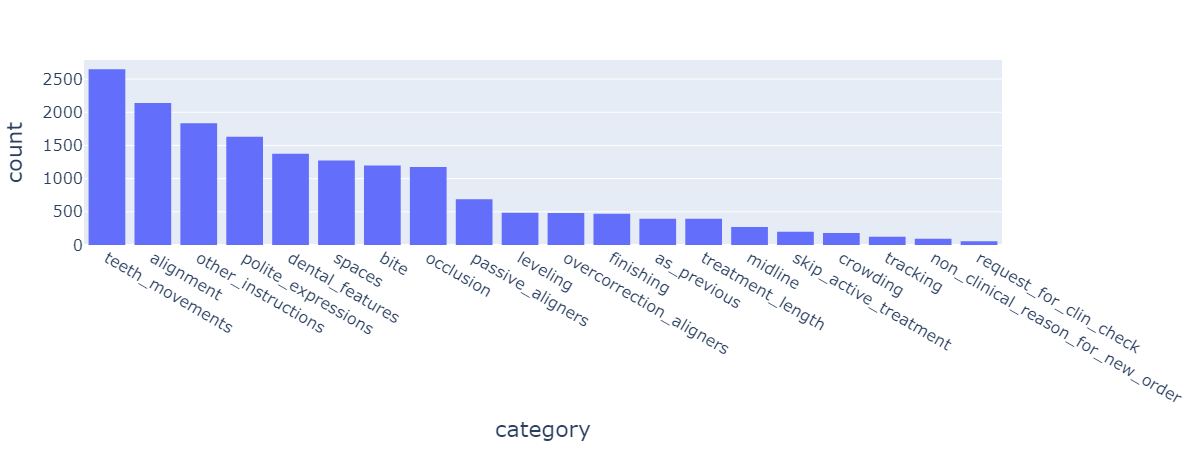
\includegraphics[scale=0.2]{images/category.png}

We split the dataset into two parts - train and validation. Train part is 80\% of the original dataset and validation is 20\%.


\section{Model}

As it has been already shown by in \cite{springer} and \cite{arxiv1} BERT, RoBERTa and other models have proven highly effective for various NLP tasks, including text classification and information extraction. Fine-tuning the mentioned transformers on our specific datasets could allow to leverage its pre-trained knowledge and adapt it to our structured output tasks.

In this article we consider the use of the following models.

\begin{table}[h!]
\centering
 \begin{tabular}{c c c} 
 \hline
 Model & Size & Details \\ [0.5ex] 
 \hline
 BERT & bert-base-uncased & 110M \\ 
 RoBERTa & roberta-base & 125M \\
 ELECTRA & electra-base & 110M \\
 GPT-4o-mini & mini & 8B \\
 GPT-4o & normal & 12B \\  [1ex]
 \hline
 \end{tabular}
\end{table}

BERT, RoBERTa and ELECTRA have been set to support the input length of 512 bytes, they have 12-layers, 768-hidden layers and 12 heads. The models are pre-trained. For all three models the classification head has been added on the top. GPT models support much longer input.

We utilize ChatGPT-4o mini, specifically focusing on its prompting capabilities. Fine-tuning ChatGPT models can be money-intensive, so we will use it to predict data through well-crafted prompts. This method allows us to assess the quality of the generated data and its utility in training other models. In real-world applications, this approach can be a cost-effective way to create labeled datasets for training smaller, task-specific models.

By using these models, we aim to cover a broad spectrum of approaches, from simple baselines to advanced LLMs. This comprehensive evaluation will help us understand the trade-offs and benefits of each method, guiding us in selecting the most effective approach for structured output tasks in natural language processing.


\section{Methods}

In this study, we use standard evaluation metrics for multi-label classification to assess the performance of our models. These metrics are well-established in the field of natural language processing and provide a quantitative basis for comparing different approaches. The primary metrics we will use include accuracy, which measures the proportion of correctly predicted labels to the total number of labels. In multi-label classification, this metric can be adapted to account for multiple labels per instance.

Precision is the ratio of true positive predictions to the total number of positive predictions. It indicates the accuracy of the positive predictions made by the model. Recall, also known as sensitivity, is the ratio of true positive predictions to the total number of actual positives. It measures the model’s ability to identify all relevant instances. The F1-score is the harmonic mean of precision and recall. It provides a single metric that balances both precision and recall, making it useful for evaluating models where there is an uneven class distribution. In particular, we use two types of F1 score - F1\_micro and F1\_macro. F1\_macro is a simple arithmetic mean over all F1 scores for classes. F1\_micro is the harmonic mean of micro precision (number of correct predictions normalized by false positives) and micro recall (number of correct predictions normalized by false negatives).

When modifying prompts for specific labels, it is crucial to monitor these metrics both overall and on a per-class basis. This allows us to identify the impact of prompt changes on individual labels and ensure that improvements in one area do not come at the expense of performance in others.

By using these metrics, we aim to provide a comprehensive evaluation of the models’ performance, enabling us to compare the effectiveness of fine-tuning and prompting methods in multi-label classification tasks.

For fine-tuning of each of the models we used the following parameters: 50 epochs, learning rate = 1e-5, optimizer AdamW.

All the fine-tuning of the models has been done on video card NVidia RTX 4070 SUPER with 12 Gb memory.

\section{Results}

After each epoch during the fine-tuning we put the model into eval mode to calculate f1 micro, f1 macro and loss on validation dataset to see the training progress.

The results of fine-tuning of BERT, RoBERTa and ELECTRA on training dataset is shown below on the pictures. F1 scores:
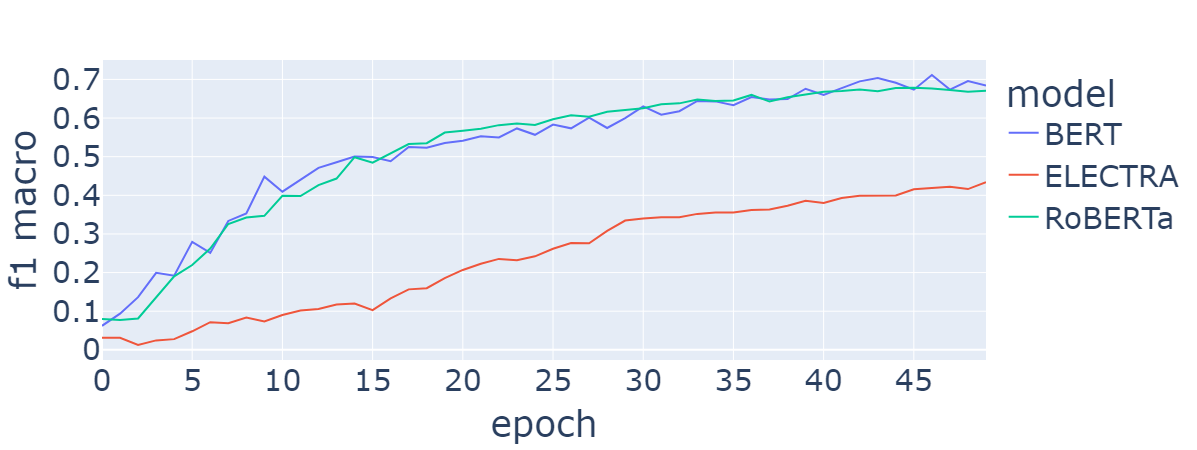
\includegraphics[scale=0.19]{images/f1scores.png}
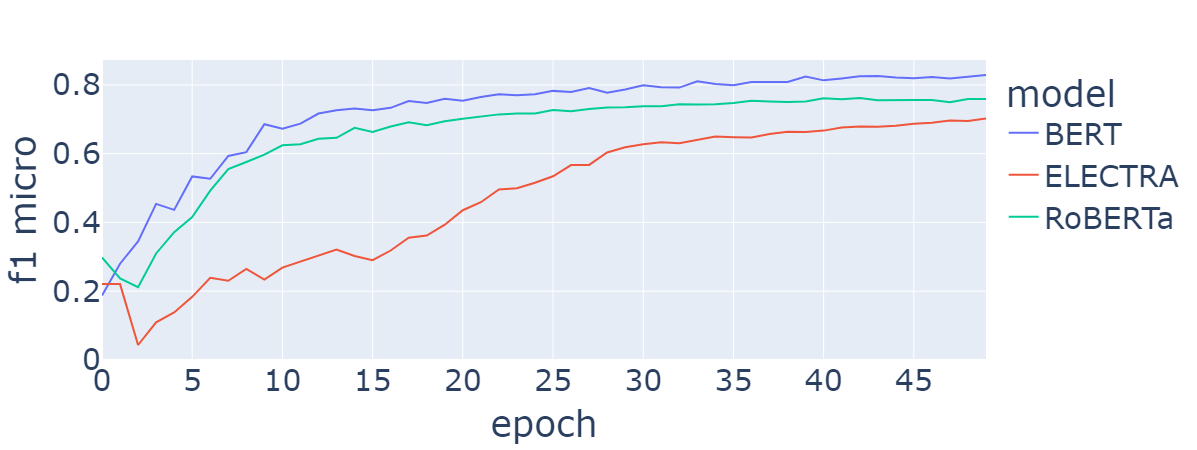
\includegraphics[scale=0.19]{images/f1scores_micro.png}

The validation loss during the training for each of the models is shown below:
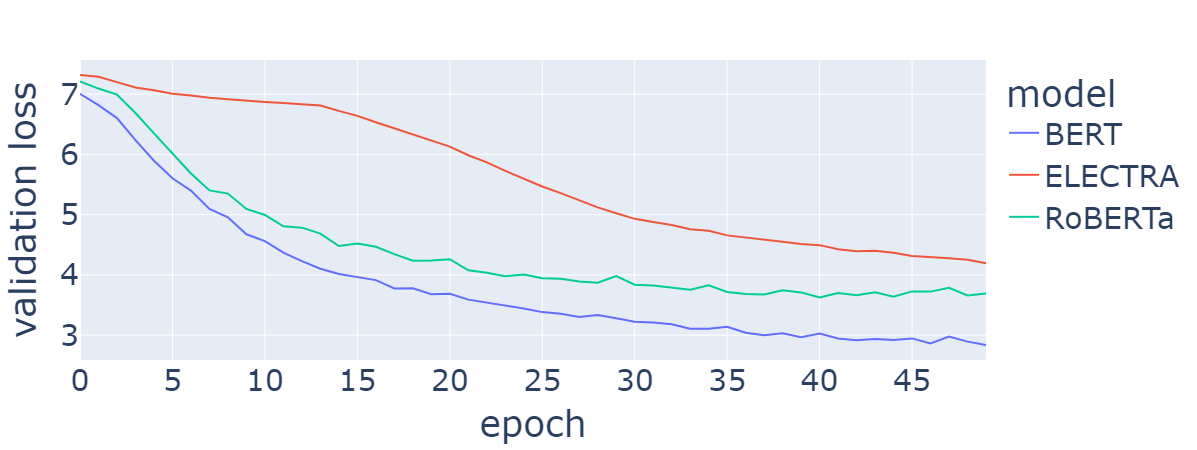
\includegraphics[scale=0.19]{images/validation_losses.png}

The resulting F1 micro and macro score values are shown below
\begin{table}[h!]
\centering
 \begin{tabular}{c c c} 
 \hline
 Model & F1 micro & F1 macro \\ [0.5ex] 
 \hline
 BERT & 0.829 & 0.711 \\ 
 RoBERTa & 0.762 & 0.678 \\
 ELECTRA & 0.702 & 0.434 \\
 GPT-4o-mini & 0.686 & 0.62 \\
 GPT-4o & N/A & 0.96 \\[1ex]
 \hline
 \end{tabular}
\end{table}

\subsection{GPT-4o-mini}
The GPT-4o-mini model achieved a mediocre score: \textbf{F1\_macro = 0.62}. This result was obtained using a prompt that was developed over six months and consisted of 20,000 tokens. Detailed metrics for each class can be found in the appendix. The prediction of one thousand phrases cost 2 dollars.

\subsection{GPT-4o}
Using this model, a final dataset of 5451 entries for training and validation was obtained. This required a colossal amount of manual work in the form of writing the prompt, predicting the entire dataset using this prompt, and then manually reviewing all predictions. After identifying errors, there was a process of correcting and improving the prompt (the final prompt occupies 20k tokens). As a result, it was possible to achieve very high quality with this model; out of 4k predictions, only 60 cases were corrected after manual adjustment. It is also worth noting the specificity of OpenAI models: even if the temperature and top-p are set to give the most repeatable result, and judging by the logs, the launch took place on the same configuration, the answers are somewhat variable, and about 200 out of 4k give different predictions. Due to the above, the quality measurement is not perfect upon repeated measurement. Running on a validation dataset of one thousand examples cost us 35 dollars and gave an \textbf{F1\_macro = 0.96}.

% Add more classes as needed

As it has been shown, the best results in classification have been shown by BERT model. It has a quicker learning rate, better converges on the dataset.

In terms of the effectiveness and costs, BERT, RoBERTa and ELECTRA could be decent and cheap option to solve the specific task such as text classification. Those models could be run not only on GPU but also on CPU configurations.

\section{Analysis} 

%Discussion of what the results mean, what they don’t mean, where they can be improved, etc. These sections vary a lot depending on the nature of the paper. (For papers reporting on experiments with multiple datasets, it can be good to repeats Methods/Results/Analysis in separate (sub)sections for each dataset.)

Fine-Tuned Models (BERT, RoBERTa, ELECTRA): The fine-tuned BERT model outperformed RoBERTa and ELECTRA on our classification tasks, achieving higher F1-micro and F1-macro scores. This suggests that BERT’s architecture, despite being a general-purpose model, adapts effectively to domain-specific tasks with sufficient labeled data. However, the relatively lower performance of RoBERTa and ELECTRA indicates that model architecture and pre-training corpora can significantly impact performance in specialized tasks. These results suggest that model selection within fine-tuning should be guided by the target task’s requirements, as even similar architectures may yield varied outcomes.

Prompt-Based Models (GPT-4o, GPT-4o-mini): ChatGPT-4o achieved high performance but at a high computational cost, while GPT-4o-mini yielded less accurate results despite significant prompt engineering efforts. This reinforces the finding that large-scale LLMs like ChatGPT-4o can produce strong performance even without retraining but require precise prompt engineering. The effort required to manually optimize prompts, coupled with model variability across prompts, reveals a need for more robust, systematic prompt generation techniques to make this approach practical for broader use cases.

\section{Conclusion} 

%Quickly summarize what the paper did, and then chart out possible future directions that anyone might pursue.

In this study, we investigated the effectiveness of fine-tuning versus prompt engineering in multi-label text classification, focusing on tasks that require structured outputs. Our experiments compared fine-tuned models like BERT, RoBERTa, and ELECTRA with prompt-based approaches using ChatGPT-4o and ChatGPT-4o-mini. Results indicated that fine-tuning generally yielded higher performance on structured output tasks, although high-performance prompt engineering approaches showed potential, particularly with larger language models.

Future research could explore:

Consider new types and architectures: There are multiple directions to investigate the new types of available models that appear every month. BERT, RoBERTa and ELECTRA are used as the most popular and representative models for research.

Optimizing Fine-Tuning Parameters: Investigating optimizers and hyperparameters for BERT-based models could further enhance performance and close existing gaps. It could be fruitful to play with amount of layers being fine-tuned, going deeper in number of unblocked layers.

Advanced Prompting Techniques: Automating prompt generation and testing alternative prompt formulations might improve consistency and accuracy for models such as ChatGPT-4o.

Cost-Effective Approaches: Developing cost-effective strategies, like hybrid fine-tuning and prompting (e.g., F\&P), could optimize the balance between computational cost and model accuracy.

Broader Task Applications: Testing both methods on more diverse tasks, particularly those requiring high interpretability, could illuminate areas where either method might uniquely excel.

Datasets Preparation: The preparation of decent dataset appears to be the main problem in resolving the tasks in a narrow domain such as orthodontics or dentistry. There is a lack of datasets on huggingface and other sources, related to orthodontics.

\section*{Known Project Limitations}

%For this section, imagine that your reader is a well-intentioned NLP practitioner who is seeking to make use of your data, models, or findings as part of a separate scholarly project, deployed system, or some other kind of real-world intervention. What should such a person know about your work? Especially important here are limitations and biases that might affect this person, their findings, their experiment participants, or the users of their product or service. The idea is that what you say here will be taken into consideration but this well-intentioned user, leading to better outcomes for everyone.
To support any practitioner intending to apply our findings in a real-world context, here are several key considerations regarding the limitations, biases, and applicability of our study.

Dataset-Specific Limitations. Our multi-label classification dataset primarily covers a specific set of structured tasks derived from orthodontic instructions. It may not generalize well to other domains where language and context differ significantly. Before applying our model to new domains, the user should consider re-evaluating or retraining on task-specific data to ensure relevance.

Prompt Dependency and Interpretability. Our results using prompt engineering—particularly with ChatGPT-4o—highlight that prompt quality directly affects model performance. This dependency introduces variability, as prompts optimized in one setting might not perform equivalently in another. This issue is particularly important in clinical or safety-critical contexts, where small differences in prompt wording could lead to inconsistent or incorrect outcomes.

Computational Costs and Budget Constraints. While ChatGPT-4o demonstrated high accuracy with careful prompt tuning, it also incurred significantly higher operational costs than the smaller models. Practitioners with limited budgets may find it challenging to sustain this model for large-scale applications. We recommend conducting a cost-benefit analysis before deployment and potentially using less expensive alternatives where possible, despite possible sacrifices in accuracy.

Model-Specific Biases. Models such as BERT, RoBERTa, and ELECTRA, while trained on diverse corpora, are prone to biases present in their pre-training datasets. For sensitive applications, practitioners should monitor for these biases, particularly in cases where predictions influence real-world decisions. Adapting the model for specific domains might require additional bias-mitigation steps, like fairness-aware training or domain-specific data augmentation.

Trade-offs Between Fine-Tuning and Prompting. Our findings suggest that while fine-tuning provides stable and often superior results for structured output tasks, it requires extensive labeled data and computational resources. Prompting, while resource-efficient, demands a meticulous design process and may not achieve consistent results across diverse task types. Practitioners should choose between fine-tuning and prompting based on their data availability, cost constraints, and need for model interpretability.

\section*{Authorship Statement}

Georgy has a long track of working with LLMs as GPT-4 and GPT-4o it is his professional occupation. He was responsible for dataset preparation and GPT models assessment. Sergey was working on fine-tuning of BERT, RoBERTa and ELECTRA models and assessment. This article is a collaborative work that started from literature review and finishing with the final paper.

% This statement is required even for singly-authored papers, because we want to know whether your project is a collaboration with people outside of the class. Our rationale for this section is that we think this is an important aspect of scholarship in general. Only in extreme cases, and after discussion with the team, would we consider giving separate grades to team members based on this statement.

% Entries for the entire Anthology, followed by custom entries
\begin{thebibliography}{}

\bibitem{kaggle}
Kaggle. Sentiment Analysis for Mental Health \textit{https://www.kaggle.com/datasets/suchintikasarkar/sentiment-analysis-for-mental-health}

\bibitem{kaggle2}
Kaggle.
Multi-Label Classification Dataset \textit{https://www.kaggle.com/datasets/shivanandmn/multilabel-classification-dataset}

\bibitem{huggingface}
Huggingface.
Mehdi Iraqi. Comparing the Performance of LLMs: A Deep Dive into Roberta, Llama 2, and Mistral for Disaster Tweets Analysis with Lora.
\textit{https://huggingface.co/blog/Lora-for-sequence-classification-with-Roberta-Llama-Mistral}

\bibitem{springer}
Arousha Haghighian Roudsari, Jafar Afshar, Wookey Lee, Suan Lee.
PatentNet: multi‑label classification of patent documents
using deep learning based language understanding.
\textit{https://link.springer.com/article/10.1007/s11192-021-04179-4}

\bibitem{arxiv1}
Zongxi Li, Xianming Li, Yuzhang Liu, Haoran Xie, Jing Li, Fu-lee Wang, Qing Li, Xiaoqin Zhong. Label Supervised LLaMA Finetuning.
\textit{https://arxiv.org/abs/2310.01208}

\bibitem{LMFSL:2020}
{Brown, Tom and Mann, Benjamin and Ryder, Nick and Subbiah, Melanie and Kaplan, Jared D and Dhariwal, Prafulla and Neelakantan, Arvind and Shyam, Pranav and Sastry, Girish and Askell, Amanda and Agarwal, Sandhini and Herbert-Voss, Ariel and Krueger, Gretchen and Henighan, Tom and Child, Rewon and Ramesh, Aditya and Ziegler, Daniel and Wu, Jeffrey and Winter, Clemens and Hesse, Chris and Chen, Mark and Sigler, Eric and Litwin, Mateusz and Gray, Scott and Chess, Benjamin and Clark, Jack and Berner, Christopher and McCandlish, Sam and Radford, Alec and Sutskever, Ilya and Amodei, Dario}
\newblock 2020.
\newblock {Language Models are Few-Shot Learners}
\newblock {\em arXiv:2005.14165}

\bibitem{PPfLLM:2021}
{Laria Reynolds, Kyle McDonell}
\newblock 2021.
\newblock {Prompt Programming for Large Language Models: Beyond the Few-Shot Paradigm}
\newblock {\em arXiv:2102.07350}

\bibitem{FTaPE:2024}
{Chanathip Pornprasit, Chakkrit Tantithamthavorn}
\newblock 2024.
\newblock {Fine-tuning and prompt engineering for large language models-based code review automation}
\newblock {\em arXiv:2402.00905}

\bibitem{LLMfTC:2024}
{Youngjin (YJ) Chae, Thomas Davidson}
\newblock 2024.
\newblock {Large Language Models for Text Classification: From Zero-Shot Learning to Instruction-Tuning}
\newblock {\em SocArXiv. doi:10.31235/osf.io/sthwk.}

\bibitem{FTaPaE:2024}
{Zezhong Wang , Luyao Ye , Hongru Wang, Boyang Xue, Yiming Du, Bin Liang, Kam-Fai Wong}
\newblock 2024.
\newblock {Fine-tuning after Prompting: an Explainable Way for Classification.}
\newblock In {\em Proceedings of the 10th SIGHAN Workshop on Chinese Language Processing (SIGHAN-10)}, pages 133–142, Bangkok, Thailand. Association for Computational Linguistics.

\bibitem{CoPEaFT:2024}
{Zhang X, Talukdar N, Vemulapalli S, Ahn S, Wang J, Meng H, Murtaza SMB, Leshchiner D, Dave AA, Joseph DF, Witteveen-Lane M, Chesla D, Zhou J, Chen B.}
\newblock 2024.
\newblock {Comparison of Prompt Engineering and Fine-Tuning Strategies in Large
Language Models in the Classification of Clinical Notes}
\newblock {\em medRxiv Preprint. 2024 Feb 8:2024.02.07.24302444. doi: 10.1101/2024.02.07.24302444.}

\bibitem{NMFTaE:2024}
{Chaozheng Wang, Yuanhang Yang, Cuiyun Gao, Yun Peng, Hongyu Zhang, Michael R. Lyu}
\newblock 2024.
\newblock {No More Fine-Tuning? An Experimental Evaluation of Prompt Tuning in Code Intelligence}
\newblock {\em 	arXiv:2207.11680}

\bibitem{AEKfLM:2020}
{Taylor Shin, Yasaman Razeghi, Robert L Logan IV}
\newblock 2020.
\newblock {\em In Proceedings of the
2020 Conference on Empirical Methods in Natural
Language Processing (EMNLP), pages 4222–4235.}

\end{thebibliography}




\end{document}
